%\chapter{Numerical Examples}
\chapter{実験・考察}

\section{実装例}

\ref{sibm:resource}で説明したリソースを使用することと、それらから習得したデータをSIBMのデータ交換環境でRDF形式のデータを得る。
避難場所情報とそれに対応するRDF述語の詳細が表\ref{table:data_rdf_predicate}のようになる。
避難場所情報とそこに作業する人の個人情報が図\ref{fig:sibm_sample}のように出力される。

\begin{table}[h]
	\begin{center}
	\begin{tabular}{| l | l | p{48mm} |}
		\hline
		\rowstyle{\bfseries}
		フィルド & RDF述語 & 内容 \\
		\hline
		位置 & geo:geopoint & 避難場所の位置 \\
		\hline
		行政区域 & sibm:administrativeAreaCode &
		都道府県コードと市区町村コードからなる、避難場所の所在する行政区を特定するためのコード \\
		\hline
		名称 & sibm:name & 避難場所の名称 \\
		\hline
		住所 & sibm:address & 避難場所の住所 \\
		\hline
		施設の種類 & sibm:facilityType & 避難場所の分類 \\
		\hline
		収容人数 & sibm:seatingCapacity & 避難施設の形態ごとの収容可能人数 \\
		\hline
		施設規模 & sibm:facilityScale & 避難施設の形態ごとの面積 \\
		\hline
		災害分類 & sibm:hazardClassification & 当該施設が対象とする災害の分類 \\
		\hline
	\end{tabular}
	\caption{避難場所情報のRDF述語の詳細}
	\label{table:data_rdf_predicate}
	\end{center}
\end{table}
	
\begin{figure}[h!]
 	\begin{center}
 		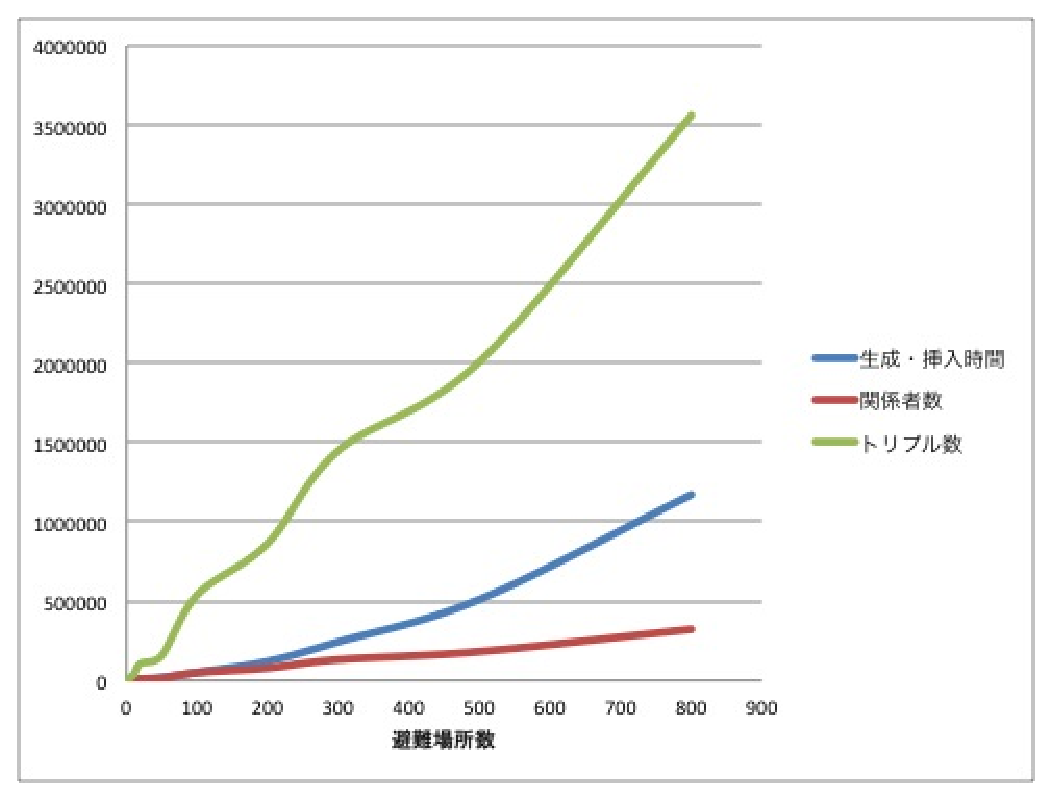
\includegraphics[width=85mm]{./images/sibm_tdb_time.eps}
 		\caption{生成時間}
 		\label{fig:sibm_data_time}
 	\end{center}
\end{figure}

\begin{figure}[h!]
\begin{center}
	\lstinputlisting{./sample/sample.txt}
  	\caption{実装例}
  	\label{fig:sibm_sample}
\end{center}
\end{figure}

\begin{table}[h]
	\begin{center}
	\begin{tabular}{| r | r | r | r | r |}
		\hline
		\rowstyle{\bfseries}
		避難場所数 & 生成・挿入時間(ms) & 関係者数 & トリプル数 & サイズ(MB) \\
		\hline
		1 & 4201 & 399 & 4411 & 192.166 \\
		\hline
		10 & 6654 & 3417 & 37753 & 193.353 \\
		\hline
		20 & 9905 & 9679 & 106795 & 195.735 \\
		\hline
		50 & 18560 & 14239 & 157435 & 197.430 \\
		\hline
		100 & 50471 & 48871 & 539187 & 265.488 \\
		\hline
		200 & 120410 & 78264 & 864110 & 315.103 \\
		\hline
		500 & 501903 & 181929 & 2009225 & 499.542 \\
		\hline
		800 & 1171083 & 322574 & 3561120 & 742.762 \\
		\hline
	\end{tabular}
	\caption{避難場所数に対する生成時間}
	\label{table:sibm_time_table}
	\end{center}
\end{table}

\section{考察}

SIBMでは、特定なパラメーターに対する避難場所情報のRDFデータセットを生成することができ、現実に近い情報の元で実験を行うことが可能である。
このセッションでは、SIBMで生成したデータセットとそのもとのパラメーターとの反映性について考察する。また、生成した情報の実用性について考察する。

\begin{table}[h]
	\begin{center}
	\begin{tabular}{| l  p{45mm} |}
		\hline
		\rowstyle{\bfseries}
		実験環境 & \\
		\hline
		Operation System & Windows 8.1 Pro 64 bits \\
		CPU & Intel core i7 3770, 4 cores 8 thread @ 3.4Ghz (Boostable up to 3.9Ghz)
		\\
		RAM & 16GB \\
		Storage & HDD \\
		Java & 1.7.0\_71 (64 bits) \\
		Apache Jena & 2.12.1 \\
		SIBM & v1.0 build 20150113 \\
		\hline
	\end{tabular}
	\caption{実験環境}
	\label{table:sibm_env}
	\end{center}
\end{table}

SIBMバージョン1で対応した入力値は避難場所の数である。SIBMが生成できる最大の数は12.5万となる。
ここでは、生成したデータをJena/TDBデータベースに挿入する時間と挿入後のデータサイズ・トリプル数について考察を行う。
入力した避難場所に対する挿入時間とデータ量が表\ref{table:sibm_time_table}になる。
避難場所の関係者数を避難場所の規模による計算される。その数によって人間情報を生成する。
表\ref{table:sibm_time_table}で示すように、避難場所の数に応じた関係者の数がわかる。

避難場所数とそれに対するデータ生成・挿入時間の関係が図\ref{fig:sibm_data_time}に示す。
生成されたデータ量(関係者数、トリプル数、データサイズ)が避難場所数に対して線形関係があることが考えられる。
だが、トリプル数/避難場所数の関係線が曲線になる。その理由は、特定な避難場所数に対して、生成しようとする関係者の数は定数ではなく、
ある範囲以内でランダムな数値で生成する。関係者情報に対するトリプル数と避難場所情報に対するトリプル数の総数では、ランダム性を持つため、
直線な関係にならないからである。

また、Jena/TDBデータベースでは、挿入するデータに対するメタデータやインデクシングすることによる発生したデータが多い。
そのため、少量データに対してもデータベースサイズが192.0MBになることがわかる\footnote{https://jena.apache.org/documentation/tdb/architecture.html}。

図\ref{fig:sibm_data_time}でわかるように、実際に発生する災害やそれに対する避難情報の増加が問題である。
例えば、北海道には約9000避難場所がある。実際に全てを使用する要求がでると、多量な情報が発生することが考えられる。そして、災害が短時間で発生することが多いため、
その短時間で多量なデータへの対策が事実な問題だとわかる。SIBMで生成するデータを使用し、その問題を解決する候補を実験することができる。
